% \iffalse
\let\negmedspace\undefined
\let\negthickspace\undefined
\documentclass[journal,12pt,twocolumn]{IEEEtran}
\usepackage{cite}
\usepackage{amsmath,amssymb,amsfonts,amsthm}
\usepackage{algorithmic}
\usepackage{graphicx}
\usepackage{textcomp}
\usepackage{xcolor}
\usepackage{txfonts}
\usepackage{listings}
\usepackage{enumitem}
\usepackage{mathtools}
\usepackage{gensymb}
\usepackage{comment}
\usepackage[breaklinks=true]{hyperref}
\usepackage{tkz-euclide} 
\usepackage{listings}
\usepackage{gvv}      
\usepackage{tikz}
\def\inputGnumericTable{}                                 
\usepackage[latin1]{inputenc}                                
\usepackage{color}                                            
\usepackage{array}                                            
\usepackage{longtable}                                       
\usepackage{calc}                                             
\usepackage{multirow}                                         
\usepackage{hhline}                                           
\usepackage{ifthen}                                           
\usepackage{lscape}
\usepackage[export]{adjustbox}

\newtheorem{theorem}{Theorem}[section]
\newtheorem{problem}{Problem}
\newtheorem{proposition}{Proposition}[section]
\newtheorem{lemma}{Lemma}[section]
\newtheorem{corollary}[theorem]{Corollary}
\newtheorem{example}{Example}[section]
\newtheorem{definition}[problem]{Definition}
\newcommand{\BEQA}{\begin{eqnarray}}
\newcommand{\EEQA}{\end{eqnarray}}
\newcommand{\define}{\stackrel{\triangle}{=}}
\theoremstyle{remark}
\newtheorem{rem}{Remark}

\begin{document}
\parindent 0px
\bibliographystyle{IEEEtran}

\vspace{3cm}

\title{}
\author{EE23BTECH11217 - Prajwal M$^{*}$
}
\maketitle
\newpage
\bigskip

% \renewcommand{\thefigure}{\theenumi}
% \renewcommand{\thetable}{\theenumi}


\section*{Exercise 9.1}

\noindent \textbf{12} \hspace{2pt}For the block diagram shown in the figure, the transfer function $\frac{Y\brak{s}}{R\brak{s}}$ is \\
\begin{figure}[h]
    \centering
    \tikzset{
    block/.style = {draw, fill=white, rectangle, minimum height=1cm, minimum width=1cm},
    plus/.style= {draw, fill=white, circle, node distance=1cm, append after command={\pgfextra \draw ($(\tikzlastnode.center) + (-0.15,0)$) -- ($(\tikzlastnode.center) + (0.15,0)$) node[above] {$+$}; \endpgfextra}},
    input/.style = {coordinate},
    output/.style = {coordinate}
}

\begin{tikzpicture}[node distance=2cm,>=latex]
    \node [input] (input) at (0,0){};
    \node [block] (block1) at (2,-2){$2$};
    \node [block] (block2) at (6,-2){$3$};
    \node [plus] (sum1) at (2,-4) {};
    \node [plus] (sum2) at (6,-4){};
    \node [block] (block3) at (4,-4) {$\frac{1}{s}$};
    \node [output] (output) at (8,-4){};
    \node [block] (block4) at (4,-6){1};
    
    \draw (input) -- node[above]{$R\brak{s}$} (2,0) to (6,0);
    \draw [->] (6,0) -- (block2);
    \draw [->] (2,0) -- (block1);
    \draw [->] (block1) -- (sum1);
    \draw [->] (sum1) -- (block3);
    \draw [->] (block3) -- (sum2);
    \draw [->] (sum2) -- node[above]{$Y\brak{s}$}(output);
    \draw [->] (block2) -- (sum2);
    \draw (7,-4) to (7,-6);
    \draw [->] (7,-6) -- (block4);
    \draw (block4) to (2,-6);
    \draw [->] (2,-6) to (sum1);  
\end{tikzpicture}

    \caption{block diagram}
    \label{fig:9.1.12.1}
\end{figure}

Solution:\\
\begin{table}[h]
    \centering
    
\begin{table}[h]
  \centering
  \begin{tabular}{|c|c|}
    \hline
    	\textbf{Symbol} & \textbf{Parameters} \\
    \hline
	  x(n) & general term of the series \\
    \hline
	  $X$(z) & Z-transform of x(n) \\
    \hline 
	  u(n) & unit step function \\
    \hline
  \end{tabular}
  \vspace{0.3cm}
  \caption{Parameters}
  \label{tab:parameters}
\end{table}

    \caption{Parameters}
    \label{tab:9.1.12.1}
\end{table}

\begin{figure}[h]
    \centering
    \usetikzlibrary{decorations.markings}
\newif\iflabrev

\begin{tikzpicture}
[
label revd/.is if=labrev,
%label revd/.default=true,
amark/.style={
            decoration={             
                        markings,   
                        mark=at position {0.5} with { 
                                    \arrow{stealth},
                                    \iflabrev \node[above] {#1};\else \node[below] {#1};\fi
                        }
            },
            postaction={decorate}
},
terminal/.style 2 args={draw,circle,inner sep=2pt,label={#1:#2}},
]

%Place the nodes
\node[terminal={above}{$R(s)$}] (a) at (0,0) {};
\node[terminal={above left}{$a$}] (b) at (1.5,0) {};
\node[terminal={above}{$b$}] (c) at (3,0) {};
\node[terminal={above right}{$c$}] (d) at (4.5,0) {};
\node[terminal={above}{$Y(s)$}] (e) at (6,0) {};
%Draw the connections
\draw[amark](a) to (b);
\draw[amark=$2$] (b) to (c);
\draw[amark=$\frac{1}{s}$] (c) to (d);
\draw[amark=$3$,label revd] (b) to[bend left=90] (d);
\draw[amark] (d) to (e);
\draw[amark=$1$] (e) to[bend left=90] (c);
\end{tikzpicture}

    \caption{signal flow graph}
    \label{fig: 9.1.12.2}
\end{figure}

Using Mason's Gain Formula for \figref{fig: 9.1.12.2},
\begin{align}
    \frac{Y\brak{s}}{R\brak{s}} & = \frac{{\sum_{i=1}^{n} P_i\Delta_i}}{{\Delta}}\\
    & = \frac{P_1\Delta_1 + P_2\Delta_2}{\Delta}\\
    & = \frac{\frac{2}{s} + 3}{1 - \frac{1}{s}}\\
    \frac{Y\brak{s}}{R\brak{s}} & = \frac{3s+2}{s-1}
\end{align}

\begin{figure}[h]
    \centering
    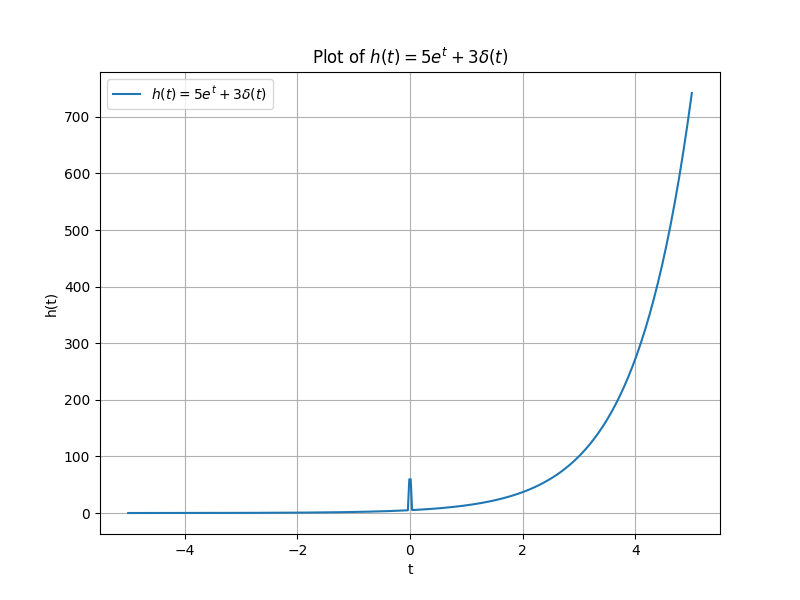
\includegraphics[width=\columnwidth]{figs/plot.png}
    \caption{signal flow graph}
    \label{fig: 9.1.12.3}
\end{figure}
\end{document}
